\documentclass[tikz,border=5pt]{standalone}
\usepackage[T1]{fontenc}
\usepackage{lmodern,amsmath,amssymb}
\usetikzlibrary{arrows.meta,calc,positioning,fit,backgrounds,shapes.geometric,matrix,decorations.pathreplacing,patterns}
\definecolor{ink}{gray}{0.08}
\definecolor{wash}{gray}{0.965}
\definecolor{soft}{gray}{0.45}
\tikzset{box/.style={draw=ink,line width=.65pt,fill=white,align=center,inner sep=4pt,outer sep=0pt,font=\small},flow/.style={draw=ink,line width=.65pt,-{Latex[length=1.8mm,width=1.3mm]},rounded corners=2pt},annotation/.style={font=\scriptsize,text=soft,align=center},groupbox/.style={draw=soft,dashed,line width=.45pt,fill=wash}}
\begin{document}
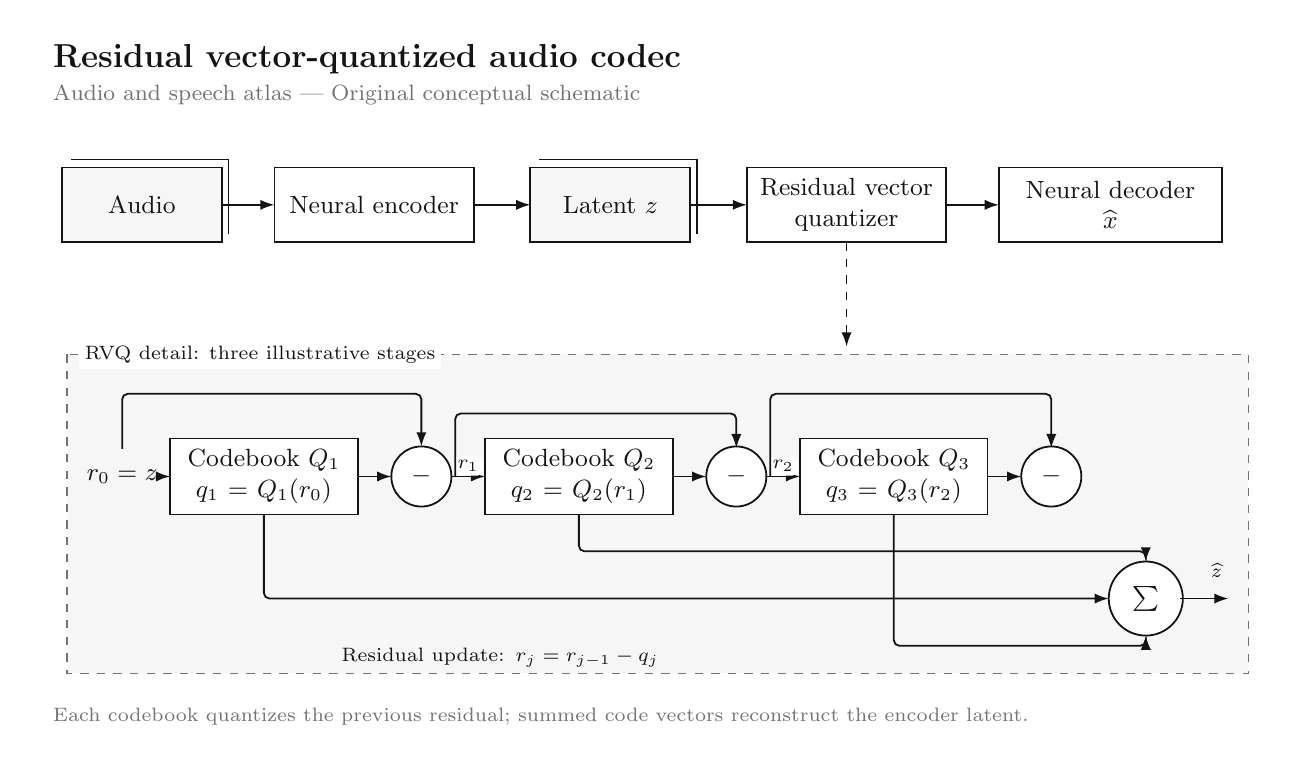
\begin{tikzpicture}[x=1cm,y=-1cm,font=\rmfamily,text=ink]

\path[use as bounding box] (0,0) rectangle (16,9);
\node[anchor=west,font=\large\bfseries] at (.2,.4) {Residual vector-quantized audio codec};
\node[anchor=west,font=\footnotesize,text=soft] at (.2,.85) {Audio and speech atlas | Original conceptual schematic};
\begin{pgfonlayer}{background}
\draw[groupbox] (0.5,4.15) rectangle (15.5,8.2);
\node[anchor=west,font=\scriptsize,fill=white,inner sep=2pt] at (0.65,4.15) {RVQ detail: three illustrative stages};
\end{pgfonlayer}
\node[box,fill=wash,minimum width=2.0cm,minimum height=0.95cm,text width=1.75cm] (audio) at (1.45,2.25) {Audio};
\draw[ink,line width=.4pt] (0.5499999999999999,1.6749999999999998) -- (2.5500000000000003,1.6749999999999998) -- (2.5500000000000003,2.625);
\node[box,minimum width=2.5cm,minimum height=0.95cm,text width=2.25cm] (enc) at (4.4,2.25) {Neural encoder};
\node[box,fill=wash,minimum width=2.0cm,minimum height=0.95cm,text width=1.75cm] (latent) at (7.4,2.25) {Latent $z$};
\draw[ink,line width=.4pt] (6.5,1.6749999999999998) -- (8.5,1.6749999999999998) -- (8.5,2.625);
\node[box,minimum width=2.5cm,minimum height=0.95cm,text width=2.25cm] (rvq) at (10.4,2.25) {Residual vector\\quantizer};
\node[box,minimum width=2.8cm,minimum height=0.95cm,text width=2.55cm] (dec) at (13.75,2.25) {Neural decoder\\$\widehat{x}$};
\node[align=center,inner sep=0pt,outer sep=0pt,font=\small,minimum width=1.2cm,minimum height=0.7cm,text width=0.95cm] (r0) at (1.2,5.7) {$r_0=z$};
\node[box,minimum width=2.35cm,minimum height=0.95cm,text width=2.1cm] (q1) at (3,5.7) {Codebook $Q_1$\\$q_1=Q_1(r_{0})$};
\node[box,circle,minimum width=0.55cm,minimum height=0.55cm,text width=0.30000000000000004cm] (sub1) at (5,5.7) {$-$};
\node[box,minimum width=2.35cm,minimum height=0.95cm,text width=2.1cm] (q2) at (7,5.7) {Codebook $Q_2$\\$q_2=Q_2(r_{1})$};
\node[box,circle,minimum width=0.55cm,minimum height=0.55cm,text width=0.30000000000000004cm] (sub2) at (9,5.7) {$-$};
\node[box,minimum width=2.35cm,minimum height=0.95cm,text width=2.1cm] (q3) at (11,5.7) {Codebook $Q_3$\\$q_3=Q_3(r_{2})$};
\node[box,circle,minimum width=0.55cm,minimum height=0.55cm,text width=0.30000000000000004cm] (sub3) at (13,5.7) {$-$};
\node[box,circle,minimum width=0.7cm,minimum height=0.7cm,text width=0.44999999999999996cm] (sum) at (14.2,7.25) {$\sum$};
\begin{pgfonlayer}{background}
\draw[flow] (audio.east) -- (enc.west);
\draw[flow] (enc.east) -- (latent.west);
\draw[flow] (latent.east) -- (rvq.west);
\draw[flow] (rvq.east) -- (dec.west);
\draw[flow] (q1.east) -- (sub1.west);
\draw[flow] (q2.east) -- (sub2.west);
\draw[flow] (q3.east) -- (sub3.west);
\draw[flow] (r0.east) -- (q1.west);
\draw[flow] (r0.north) -- (1.2,4.65) -- (5,4.65) -- (sub1.north);
\draw[flow] (sub1.east) -- (q2.west) node[midway,above,fill=white,inner sep=1.5pt,font=\scriptsize] {$r_1$};
\draw[flow] (sub2.east) -- (q3.west) node[midway,above,fill=white,inner sep=1.5pt,font=\scriptsize] {$r_2$};
\draw[flow] (q1.south) -- (3,7.25) -- (sum.west);
\draw[flow] (q2.south) -- (7,6.65) -- (14.2,6.65) -- (sum.north);
\draw[flow] (q3.south) -- (11,7.85) -- (14.2,7.85) -- (sum.south);
\end{pgfonlayer}
\draw[flow] (5.43,5.7) -- (5.43,4.9) -- (9,4.9) -- (9,5.34);
\draw[flow] (9.43,5.7) -- (9.43,4.65) -- (13,4.65) -- (13,5.34);
\draw[flow] (14.63,7.25) -- (15.25,7.25);
\node[align=center,anchor=center,font=\scriptsize,text=ink,text width=1.0cm] at (15.1,6.9) {\mbox{$\widehat z$}};
\node[align=center,anchor=center,font=\scriptsize,text=ink,text width=8cm] at (6.0,8.0) {Residual update: \mbox{$r_j=r_{j-1}-q_j$}};
\draw[flow,dashed] (10.4,2.725) -- (10.4,4.05);
\node[anchor=west,align=left,font=\scriptsize,text=soft,text width=15.6cm] at (.2,8.75) {Each codebook quantizes the previous residual; summed code vectors reconstruct the encoder latent.};
\end{tikzpicture}
\end{document}
